\documentclass[10pt]{exam}
\usepackage[hon]{template-for-exam}
\usepackage{endnotes,graphicx}
\usepackage{tikz,graphicx,enumitem,multicol,float,my-tikz-clipart,silence,cclicenses,tikzpingus}
\graphicspath{{./figures/}}
\WarningFilter{latex}{Label `part}
\WarningFilter{latex}{There were multiply-defined labels}
\usetikzlibrary{arrows.meta}

\footer{}{\thepage}{\sc \myclass}


%\def\answer#1{\footnotetext{#1}}
%\def\myquestion{\item\stepcounter{footnote}}

\def\enoteheading{}
\def\answer#1{\endnotetext{#1}}
\def\theanswers{\theendnotes}
\def\myquestion{\item\stepcounter{endnote}}

\newenvironment{myquestions}{
  \begin{multicols}{2}\begin{enumerate}[resume]
}{
  \end{enumerate}\end{multicols}
}
\makeatletter
\patchcmd{\enit@setresumekeys}{\def}{\gdef}{}{}
\patchcmd{\enit@setresumekeys}{\def}{\gdef}{}{}
\makeatother

\newcommand{\myheading}[1]{\uplevel{\section*{#1}}
}
\newcommand{\mysubheading}[1]{\uplevel{\subsection*{#1}}
}

%uncomment if running Pandoc
% \renewcommand{\myheading}[1]{{\section*{#1}}}
% \renewcommand{\mysubheading}[1]{\subsection*{#1}}

\title{Chapter 4-5 Homework B (Friction \& Forces at an Angle)}
\author{Rohrbach}
\date{\today}

\def\mymaketitle{
  \begin{flushleft}
    {\LARGE \textbf \mytitle \par}
  \end{flushleft}
}

\newcommand{\bs}[2]{\textbf{#1} (\sc #2 Points)}


\newcommand{\GFig}[2]{  
  \begin{figure}[H]
    \centering
    \includegraphics[width=#2]{11_#1_Figure.jpg}
    \caption{Giancolli Figure 11-#1.}
    \label{11-#1}
  \end{figure}
}


\begin{document}
\maketitle

  \hfill
  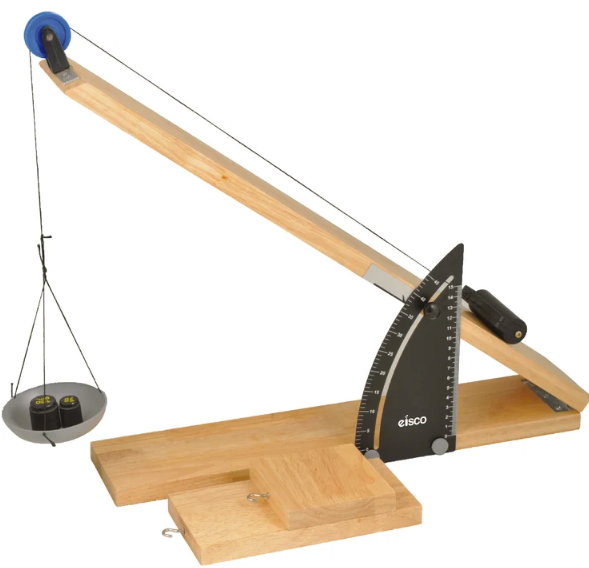
\includegraphics[height=2.5in]{OpenStaxImages/eisco} 
  \hfill\,


  \vfill
  \hrule
  \vspace{0.2em}

    \begin{table}[h]
    \centering
    \begin{tabular}{lcc}
      \hline
      \textbf{System}        & $\mu_s$ & $\mu_k$ \\
      \hline
      Rubber on dry concrete   & 1.0   & 0.7   \\
      Rubber on wet concrete   & 0.7   & 0.5   \\
      Wood on wood             & 0.5   & 0.3   \\
      Waxed wood on wet snow   & 0.14  & 0.1   \\
      Metal on wood            & 0.5   & 0.3   \\
      Steel on steel (dry)     & 0.6   & 0.3   \\
      Steel on steel (oiled)   & 0.05  & 0.03  \\
      Teflon on steel          & 0.04  & 0.04  \\
      Shoes on wood            & 0.9   & 0.7   \\
      Shoes on ice             & 0.1   & 0.05  \\
      Ice on ice               & 0.1   & 0.03  \\
      Steel on ice             & 0.04  & 0.02  \\
      \hline\hline
    \end{tabular}
    \caption{(OpenStax Table 5.1) Coefficients of Static and Kinetic Friction}
    \label{mu}
  \end{table}


  \hrule

  
  \section*{Equations}

  \begin{align*}
    \Sigma \vec{F} &= m\vec{a} &
    F_G &= mg &
    F_{f,s} &\le \mu_s F_N &
    F_{f,k} &= \mu_k F_N
  \end{align*}
  
  \hrule

  \section*{Selected Answers}

  \renewcommand{\enotesize}{\normalsize}
  \renewcommand{\enoteformat}{%
    \leftskip=1.8em
    \makebox[0pt][r]{\theenmark. }%
  }

  \hfill

  \begin{multicols}{2}
    \theanswers
  \end{multicols}



\pagebreak

\noindent
\textit{Questions and figures are from OpenStax} College Physics, \textit{2nd ed (Chapter 5) unless otherwise noted.}

\section*{Friction}

\begin{myquestions}

\myquestion
    (P1) A physics major is cooking breakfast when he notices that the frictional force between his steel spatula and his Teflon frying pan is only 0.200 N. Knowing the coefficient of kinetic friction between the two materials, he quickly calculates the normal force. What is it? (Use the coefficients of friction provided in Table~\ref{mu} on the front of this packet) \answer{\SI{5.00}{N}}

  \myquestion
    (P4) Suppose you have a 120-kg wooden crate resting on a wood floor. (a) What maximum force can you exert horizontally on the crate without moving it? (b) If you continue to exert this force once the crate starts to slip, what will the magnitude of its acceleration then be? (Use the coefficients of friction provided in Table~\ref{mu})  \answer{(a) \SI{588}{N}; (b) \SI{1.96}{m/s^2}}

  \myquestion (Original Question)
    A 7-kg wood box is pushed across a horizontal wood floor.  (a) Once there is no longer any applied force, what is the box's acceleration? (b) How far does the box slide before coming to a complete stop if its initial velocity is 4.4~m/s? \answer{(a) \SI{-2.94}{m/s^2}; (b) \SI{3.29}{m}}



  \myquestion \label{ModAtwood}
    (Original question) A metal block of mass $m_1=25$~kg rests on a horizontal wood table. The block is connected by a light, inextensible string that passes over a frictionless pulley to a hanging block of mass $m_2=10$~kg. \answer{(b) \SI{0.70}{m/s^2}; (c) \SI{91}{N}}
    %
    \begin{parts}
      \part Draw a free-body diagram for each block.
      \part Determine the acceleration of the system.
      \part Find the tension in the string.
    \end{parts}

    \tikzstyle{box}=[rounded corners,draw,minimum height=1cm]
    \begin{figure}[H]
      \centering
      \begin{tikzpicture}
        \node[box,minimum width=1.5cm] (one) at (0,0) {$m_1$};
        \node[box] (two) at (3.75,-3) {$m_2$};
        \draw[very thick] (one.east) -- (3.5,0) arc (90:0:0.25) -- (two);
        \fill[pattern=north east lines] (-3,-0.5) rectangle
          ++(6,-0.25);
        \draw (-3,-0.5) -- 
          ++(6,0) coordinate (edge) -- 
          ++(0,-1);
        \draw (edge) -- (3.5,-0.25) circle (0.25);
      \end{tikzpicture}
      \caption{(Original Diagram) Figure for problem~\ref{ModAtwood}.}
    \end{figure}

  % \myquestion
  %   (OpenStax Ch 5, P5) (a) If half of the weight of a small 1,000-kg utility truck is supported by its two rubber drive wheels, what is the magnitude of the maximum acceleration it can achieve on dry concrete? (b) Will a 45-kg metal cabinet lying on the wooden bed of the truck slip if it accelerates at this rate? %(c) Solve both problems assuming the truck has four-wheel drive. 
  %   \answer{(a) \SI{4.90}{m/s^2}; (b) will not slip}%; (c) \SI{9.8}{m/s^2} and will slip}

\end{myquestions}


\pagebreak

\section*{Forces at an Angle}


\begin{myquestions}
  \myquestion 
    (P21 with significant modification) A contestant in a winter sporting event pushes a 45.0-kg block of ice across a frozen lake as shown in Figure~\ref{5-21}(a).  A second contestant pulls it as in Figure~\ref{5-21}(b).  Both contestants exert a force $F=15$~N.  Calculate the acceleration of and normal force on each block. \answer{(a) \SI{0.302}{m/s^2}, \SI{435}{N}; (b) \SI{0.302}{m/s^2}, \SI{447}{N}}

    \begin{figure}[H]
      \centering
      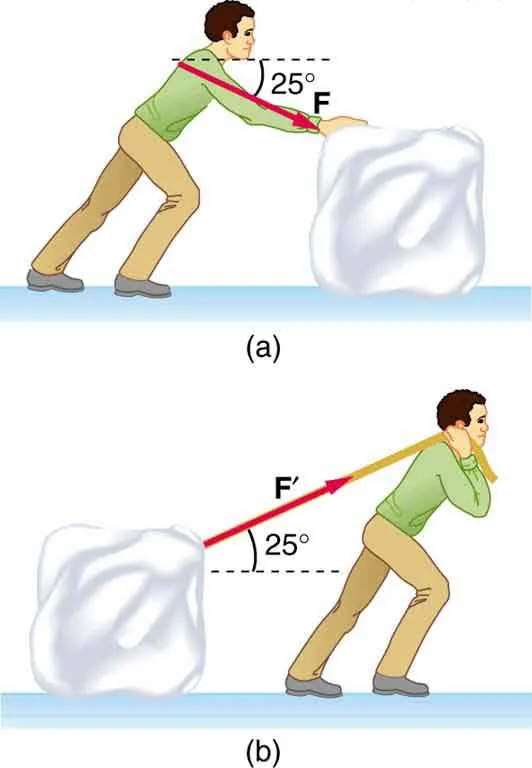
\includegraphics[height=2.3in]{OpenStaxImages/5-21.jpg}
      \caption{(OpenStax Fig 5.21) Which method of sliding a block of ice requires less force—(a) pushing or (b) pulling at the same angle above the horizontal?}
      \label{5-21}
    \end{figure}

  \myquestion
    (P11a) Calculate the acceleration of a 70-kg skier heading down a $10^\circ$ slope, assuming the coefficient of friction for waxed wood on wet snow from Table~\ref{mu}. \answer{0.737 m/s$^2$}

  \myquestion (Ch 4, P57 from Giancolli \textit{Physics: Principles with Applications}, 7th ed.) \answer{\SI{3.67}{m/s^2}}
    The block shown in Figure~\ref{G4-59} has mass $m=7.0$~kg and lies on a fixed smooth frictionless plane tilted at an angle $\theta=22^\circ$ to the horizontal. Determine the acceleration of the block as it slides down the plane.    

        \begin{figure}[H]
          \centering
          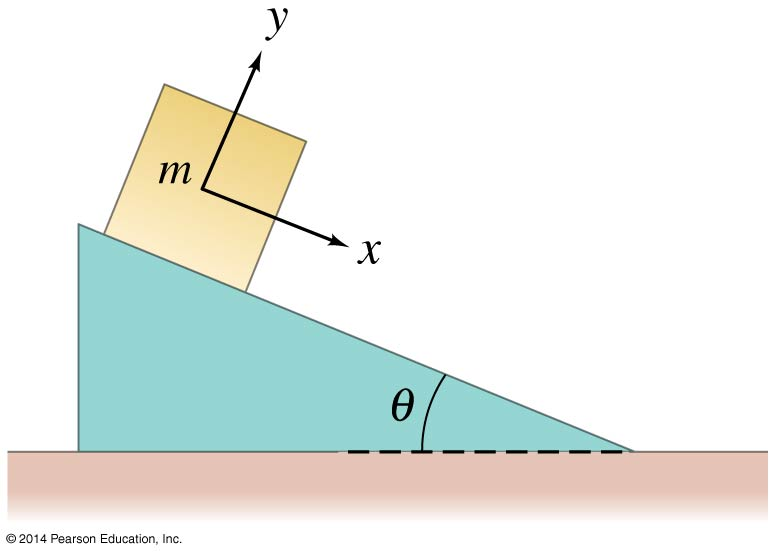
\includegraphics[width=2.5in]{OpenStaxImages/Giancolli4-59.jpg}
          \caption{Fig 4-59 from Giancolli}
          \label{G4-59}
        \end{figure}





  % \myquestion
  %   (OpenStax Ch 5, P8) Show that the acceleration of any object down a frictionless incline that makes an angle $\theta$ with the horizontal is $a=g\sin\theta$. (Note that this acceleration is independent of mass.)   
  
  % \myquestion
  %   (OpenStax Ch 5, P9) Show that the acceleration of any object down an incline where friction behaves simply (that is, where $f_k=\mu_k N$) is $a=g\left( \sin\theta - \mu_k \cos\theta \right)$.  Note that the acceleration is independent of mass and reduces to the expression found in the previous problem when friction becomes negligibly small ($\mu_k=0$).

  % \myquestion
  %   (OpenStax Ch 5, P10) Calculate the deceleration of a snow boarder going up a $5.0^\circ$, slope assuming the coefficient of friction for waxed wood on wet snow. The result of the previous problem may be useful, but be careful to consider the fact that the snow boarder is going uphill. \answer{\SI{1.83}{m/s^2}}

  

\end{myquestions}

\pagebreak

\section*{Conceptual Questions}

  \begin{enumerate}[resume]
    \myquestion (Original Question) Look above at Figure~\ref{5-21} on the previous page.  This time, assume that friction is \emph{not} negligible.  Which method of moving the block would be easier: pulling from in front or pushing from the back? Explain. \vs 
    \myquestion (Original Question) One block sits at rest on a level surface while a second identical block sits at rest on an incline.  In which case is the normal force larger?  Why? \vs 
  \end{enumerate}


\hrule


\section*{Additional Practice}
These problems are not required and are not bonus. Worked out solutions are available on Schoology.
  
\begin{myquestions}
  

    \myquestion
      (Ch 4, P37 from Giancolli \textit{Physics: Principles with Applications}, 7th ed.) A force of 35.0~N is required to start a 6.0-kg box moving across a horizontal concrete floor.  (a) What is the coefficient of static friction between the box and the floor?  (b) If the 35.0-N force continues, the box accelerates at \SI{0.60}{m/s^2}. What is the coefficient of kinetic friction? \answer{(a) $\mu_s=0.60$ (b) $\mu_k=0.53$}

    \myquestion (Ch 4, P56 from Giancolli) \answer{104 N; $\mu_k=0.475$}
      A 25.0-kg box is released on a $27^\circ$ incline and accelerates down the incline at \SI{0.30}{m/s^2}. Find the friction force impeding its motion. What is the coefficient of kinetic friction?

    % \myquestion
    %     (Ch 4, P49 from Giancolli, modified) Two crates of mass 65~kg and 125~kg are in contact and at rest on a horizontal surface (Figure~\ref{G4-47}).  A 650-N force is exerted on 65-kg crate.  Calculate (a) the acceleration of the system and (b) the force that each crate exerts on the other.  (c) Repeat with the crates reversed. \answer{(a) \SI{3.42}{m/s^2} (b) \SI{427.5}{N} (c) \SI{3.42}{m/s^2} and \SI{22.3}{N} }

    %     \begin{figure}[h]
    %       \centering
    %       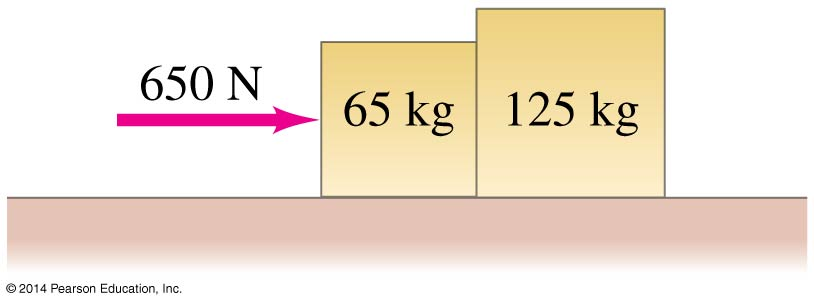
\includegraphics[width=2in]{OpenStaxImages/Giancolli4-57.jpg}
    %       \caption{Fig 4-47 from Giancolli}
    %       \label{G4-47}
    %     \end{figure}


\end{myquestions}

\hrule

\section*{Bonus}

You will be given bonus if you complete these problems \emph{on a separate sheet of paper}
  
\begin{myquestions}


  \myquestion \label{b3} (P11b)
     A 70-kg skier is heading down a slope.  Assuming the coefficient of friction for waxed wood on wet snow from Table~\ref{mu}, find the angle of the slope down which the skier could coast at a constant velocity. \answer{$5.71^\circ$}

  \myquestion (P12) If an object is to rest on an incline without slipping, friction must equal the component of the weight parallel to the incline. Show that the maximum angle of an incline above the horizontal for which an object will not slide down is $\theta = \tan^{-1} \left( \mu_s \right)$. Assume $a = 0$ and static friction has reached its maximum value.
  
\end{myquestions}

  
\end{document}